%\graphicspath{{~/Pictures/Screenshots/}} % path to graphics
\graphicspath{{./img/}} % path to graphics

\chapter{Разработка проекта и системы сборки}
\section{Файл README.md}
README --- это первый файл, который нужно читать, получив доступ к проекту
на Github или любой Git-хостинговой площадке. Этот файл в первую очередь
и предлагается вниманию пользователя, когда он открывает здесь репозиторий
того или иного проекта. Такой файл содержит кучу полезной информации, так что
его вполне можно рассматривать как справочное руководство по проекту.\par
Расширение \texttt{.md} --- это сокращение от слова markdown.\par
Markdown — язык текстовой разметки, созданный писателем и блогером
Джоном Грубером. Он предназначен для создания красиво оформленных текстов
в обычных файлах формата TXT.\par
Для данного проекта был написан такой README-файл:

\begin{verbatim}
# TelegramBot_Queue
Телеграмм бот, позволяющий отслеживать и контролировать очередь
на сдачу работ в университете. Данный чат-бот может значительно
облегчить тайм-менджмент преподователей и студентов.
# How to install 
1. Для начала необходимо усановить [Python3]
(https://www.python.org/downloads/).
2. `python3 setup.py` - установим необходимые зависимости.
3. `python3 main.py` - запуск бота.
4. Теперь необходимо зайти в приложение Telegramm
для взаимодействия с ботом.
\end{verbatim}

\section{Система сборки}
Setuptools --- это полнофункциональная, активно поддерживаемая
и стабильная библиотека, предназначенная для облегчения упаковки
проектов на Python.

Это помогает разработчикам легко обмениваться повторно используемым кодом
(в виде библиотеки) и программами (например, инструментами CLI / GUI,
реализованными на Python), которые могут быть установлены с помощью pip
и загружены в PyPI.

\begin{lstlisting}[language=Python
	, caption=\leftline{Текст файла setup.py}
	, label=lst:setup]
from setuptools import setup, find_packages
from os import path

here = path.abspath(path.dirname(__file__))
long_description = open(here+"/"+"README.md", 'r').read()

if __name__ == "__main__":
	setup(
		name="BotQueueTg",
		version="1.0.0",
		description="Python project implementing\
			a bot queue in the telegram social network",
		packages=find_packages(
			exclude=['venv']
		),
		install_requires=['pyTelegramBotAPI']
	)
\end{lstlisting}

\section{Docstrings}
Строки документации (docstrings) в Python --- это строковые литералы,
которые пишутся сразу после определения функции, метода, класса или модуля.

\section{Сборка документации проекта}
С помощью модуля doc, напишем код, который генерирует документацию по проекту

\begin{lstlisting}[language=Python
, caption=\leftline{doc.py}
, label=lst:doc]
import pdoc

modules = ['main.py', 'db.py']  # Публичные субмодули импортируются автоматически
context = pdoc.Context()
modules = [pdoc.Module(mod, context=context)
for mod in modules]
pdoc.link_inheritance(context)


def recursive_htmls(mod):
yield mod.name, mod.html()
for submod in mod.submodules():
yield from recursive_htmls(submod)


for mod in modules:
for module_name, html in recursive_htmls(mod):
with open('doc\ ' + module_name + ".html", 'w', encoding="utf-8") as f:
f.write(html)

\end{lstlisting}

Пример сгенерированный документации\ref{fig:doc}.
\begin{figure}[h!tp]
\centering
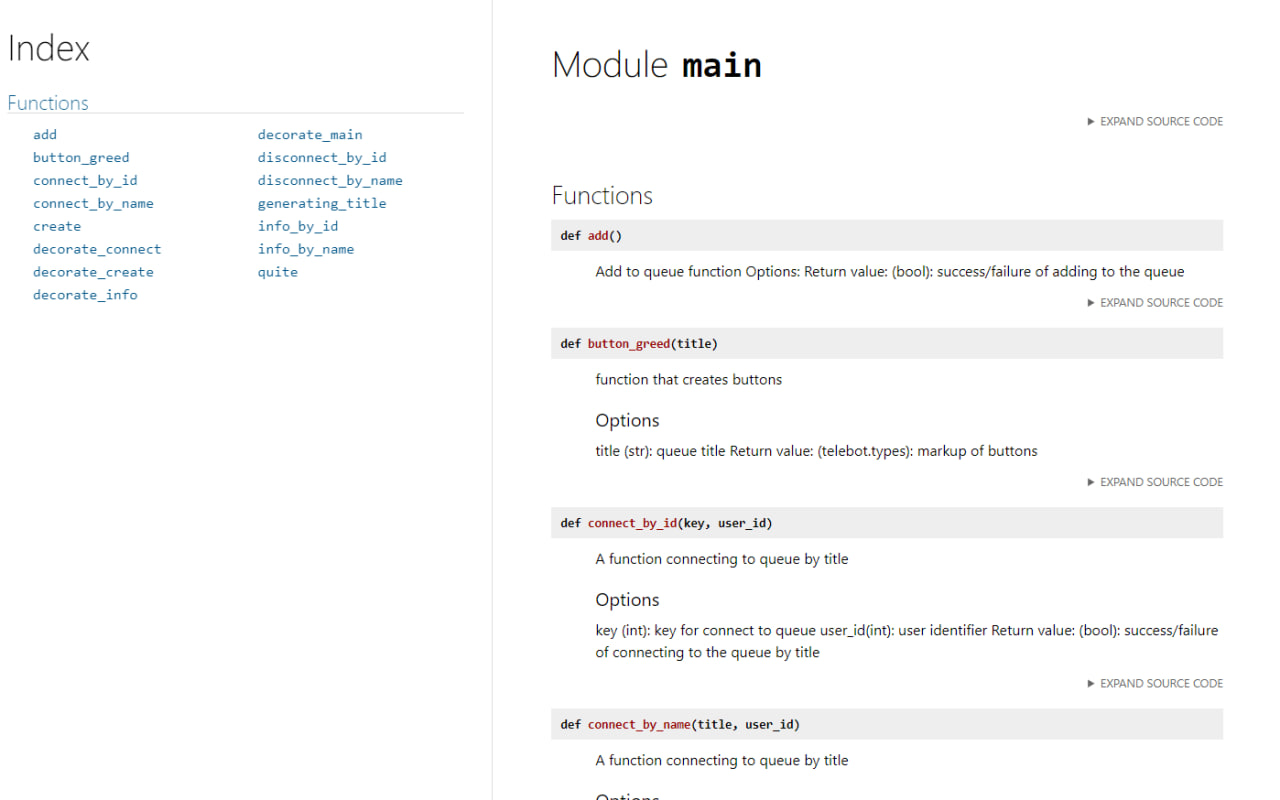
\includegraphics[width=0.55\textwidth]{doc}
\caption{Пример интерфейса}
\label{fig:doc}
\end{figure}
